\documentclass[11pt,reqno]{beamer}
\usepackage[utf8x]{inputenc}
\usetheme{Dresden}
\usecolortheme{beaver}


\usepackage{amsmath}
\usepackage{amsfonts}
\usepackage{array}
\usepackage{graphicx}
\usepackage{tabularx}
\usepackage{hyphenat}

\setbeamertemplate{navigation symbols}{}


\title{An Introduction to Bond Graph Modelling}
\subtitle{12th International CellML Workshop}
\author{Peter Cudmore\inst{1,2}}
\titlegraphic{
\includegraphics[width=1.75cm]{PRIMARY_A_Vertical_Housed_RGB.png}}
\institute[]{\tiny
\inst{1} Systems Biology Laboratory, School of Mathematics and Statistics and Department of Biomedical Engineering, University of Melbourne, Parkville, Victoria 3010 \and
\inst{2} ARC Centre of Excellence in Convergent Bio-Nano Science and Technology, Melbourne school of Engineering, University of Melbourne, Parkville, Victoria 3010}
\date{}

\graphicspath{{../../images/}}

\newcommand{\D}[2]{\frac{\mathrm{d} #1}{\mathrm{d} #2}}
\newcommand{\e}{\mathrm{e}}
\newcommand{\I}{\mathrm{i}}
\renewcommand{\mod}[1]{\left|#1\right|}
\newcommand{\DD}[2]{\frac{\mathrm{d}^2 #1}{\mathrm{d} #2^2}}
\newcommand{\bigO}[1]{\text{O}\left(#1\right)}
\renewcommand{\P}[2]{\frac{\partial #1}{\partial #2}}
\renewcommand{\Re}{\operatorname{Re}}
\renewcommand{\Im}{\operatorname{Im}}
\newcommand{\EX}{\mathbb{E}}
\newcommand{\df}[1]{\mspace{2mu}  \mathrm{d}#1}
\newcommand{\reals}{\mathbb{R}}
\newcommand{\complex}{\mathbb{C}}
\newcommand{\conj}[1]{\overline{#1}}

\AtBeginSection[] { 
	\begin{frame}
	\tableofcontents[currentsection,hideallsubsections] 
	\addtocounter{framenumber}{-1} 
\end{frame}
}
\begin{document}
	\begin{frame}
	\titlepage
	\addtocounter{framenumber}{-1} 
\end{frame}
\section{Introduction}
\begin{frame}
\frametitle{Goals of this talk}
My first aim is to convince you that:
\begin{itemize}
	\item Bond graphs are a `natural' way to model energy distribution across networked systems
	\item Bond graphs are very useful for modelling multi-domain systems.
\end{itemize}

\vspace{10pt}

I will then introduce some basic bond graph components.
\vspace{10pt}

Finally, I will talk briefly about bond graph research at the Systems Biology Lab.
\vspace{10pt}

Slides are online: \url{https://github.com/peter-cudmore/}
\end{frame}

\begin{frame}
\frametitle{Bond Graph History}
\begin{figure}
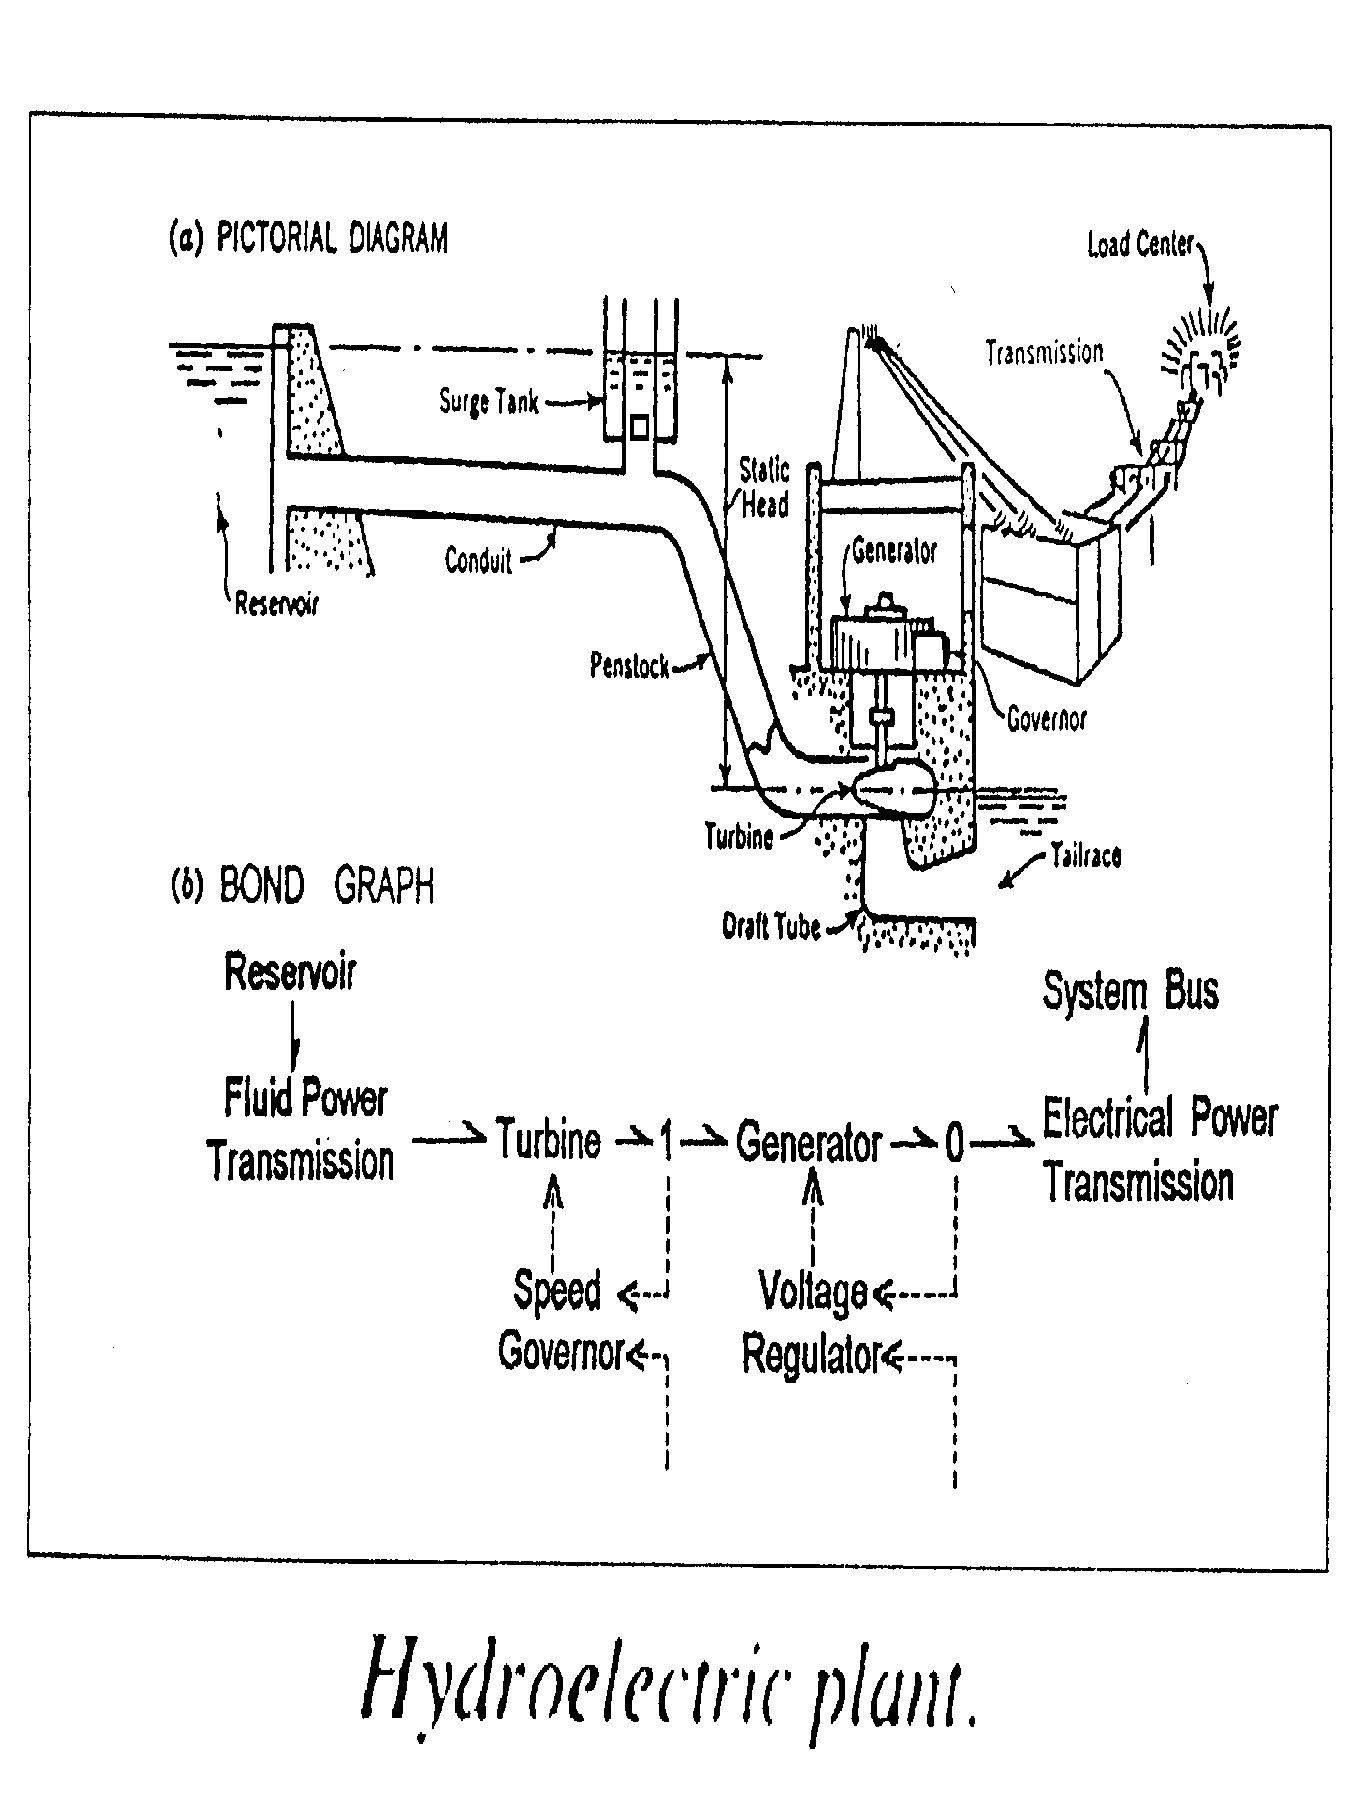
\includegraphics[height=0.6\textheight, width=0.7\linewidth]{hydro.jpg}
\end{figure}
Bond graphs were invented by Henry Paynter~\cite{payter2000} in 1959.
\end{frame}
\begin{frame}
\frametitle{Bond Graphs Today}
:
\begin{itemize}
	\itemsep1em
	\item Bond graph modelling is used both explicitly and implicitly in mechatronics, power systems engineering and control theory.
	\item Bond graphs tie deeply into classical mechanics and thermodynamics.
	\item Recent advances have included bond graph to models of biochemical reactions~\cite{Gaw2017a, Gaw2017b, Gaw2014}.
\end{itemize}
\end{frame}

\section{Power distribution networks}
\begin{frame}
\frametitle{The Fundamental Law: Conservation of Energy}
\begin{quotation}
	There is a fact, or if you wish, a law, governing all natural phenomena that are known to date. There is no known exception to this law—it is exact so far as we know. The law is called the conservation of energy.
\end{quotation}

- Richard Feynman, 1961~\cite{Feynman1961}.
\end{frame}
\begin{frame}{Energy Networks}
Bond Graphs model systems that:
\begin{itemize}
	\item use energy as the core currency.
	\item can be decomposed into functionally discrete subsystems.
	\item transfer of energy between subsystems.
\end{itemize}
\vspace{1cm}
Hence Bond Graphs have a network structure!
\end{frame}
\begin{frame}
\frametitle{Implied Network Structure}
\begin{figure}
	\centering
	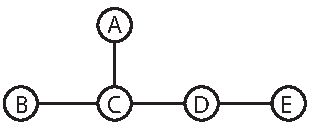
\includegraphics{network_1.pdf}
	\caption{An Energy Network}
\end{figure}
Nodes represent subsystems that act upon energy.

\vspace{5pt}

Edges represent transfer of energy between subsystems.
\end{frame}

\begin{frame}
\frametitle{Open Systems}
\begin{figure}
\centering
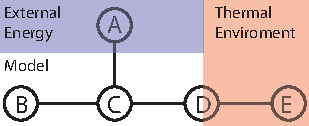
\includegraphics{network_2.pdf}
\end{figure}
\centering
is modelled as
\begin{figure}
\centering
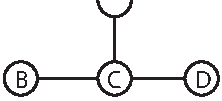
\includegraphics{network_2a.pdf}
\end{figure}
\end{frame}
\begin{frame}
\frametitle{Power}
\begin{figure}
	\centering
	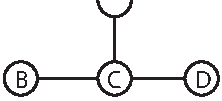
\includegraphics{network_2a.pdf}
\end{figure}
Power is exchanged between subsystems $B,C,D$. \\
\vspace{5pt}

Power is represented in terms of \emph{effort} $e$ and \emph{flow} $f$ such that 
\[
\text{Power} = \text{effort}\times\text{flow} \qquad \iff \qquad P=ef
\]
\end{frame}
\begin{frame}
\frametitle{Domain Specific Power}
\begin{figure}
\nohyphens{\scriptsize
	\renewcommand{\arraystretch}{1.5}
	\begin{tabular}{p{1.5cm} | p{1.75cm} | p{1.75cm} |p{1.75cm} | p{1.75cm}|}
		Domain & $q$ & $f = \dot{q}$ & $p$ & $e = \dot{p}$\\
		\hline
		Translational Mechanics & position & velocity & momentum & force\\
		\hline 
		Rotational Mechanics & angle & angular velocity & angular momentum & torque\\
		\hline 
		Electronics & charge  & current & flux linkage & voltage\\
		\hline 
		Hydraulics & volume & flow & pressure momentum & pressure\\
		\hline 
		Thermo-dynamics & entropy & entropy flow & temperature momentum & temperature\\
		\hline 
		Chemistry & moles & molar flow& chemical momentum & chemical potential\\
		\hline 
\end{tabular}}
\caption{State space $(q,p)$ and phase space $(e,f)$ variables \cite{Karnopp, baez}.}
\end{figure}

\end{frame}
\begin{frame}
\frametitle{Network Structure with 2-variable Edges}
The power transferred into $B$ is given by $e_1\times f_1$.
\begin{figure}
	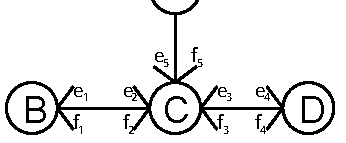
\includegraphics{portbondgraph.pdf}
\end{figure}
Hence the energetic behaviour of the $B$ subsystem can be specified by
$\Phi_B(e_1,f_1)= 0$. Similarly for the $C$ and $D$ subsystems.\\
\vspace{10pt}

\emph{$\Phi_B$ describes some kind of physical process like energy storage or dissipation.}
\end{frame}
\begin{frame}
\frametitle{Directed Network Structure}
\only<1>{
\begin{figure}
	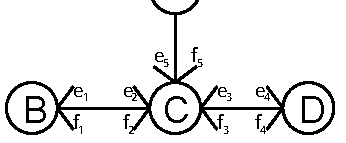
\includegraphics{portbondgraph.pdf}
\end{figure}
Conservation of Energy must hold across edges, hence
\[
e_1f_1 +e_2f_2 = 0, \qquad e_3f_3 +e_4f_4 = 0.
\]}
\only<2>{
\begin{figure}
	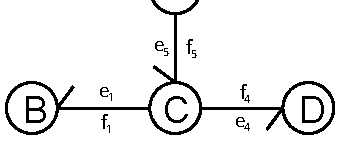
\includegraphics{portbondgrapha.pdf}
\end{figure}
We choose a sign, and denote the direction of positive $f$ by a half-arrow.
Hence
\[
e_2 = e_1, \quad f_2 = -f_1, \qquad e_3 = e_4, \quad f_3 = -f_4,
\]
which are used to update the co-ordinates of $\Phi_B,\Phi_C$ and $\Phi_D$.
}
\only<3>{
\begin{figure}
	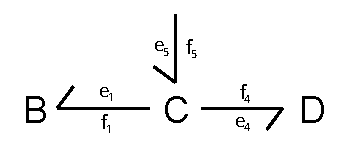
\includegraphics{bondgraph.pdf}
\end{figure}Discard the extra circles, we get an acausal bond graph.}

\end{frame}
\begin{frame}
\frametitle{Key Features of a Bond Graph}
\begin{figure}
	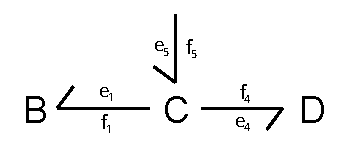
\includegraphics{bondgraph.pdf}
\end{figure}
	\begin{itemize}
		\item Subsystem defined by constitutive relations $\Phi_B(e_1,f_1) = 0$  etc.
		\item Bonds show \emph{shared variables} through which power is balanced.
		\item Half arrows indicate positive $f$ (sign convention).
\end{itemize}
\end{frame}
\begin{frame}
\frametitle{Strengths and Weaknesses}
\begin{figure}
	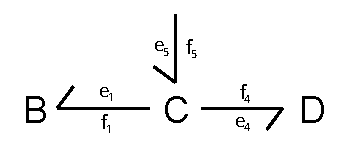
\includegraphics{bondgraph.pdf}
\end{figure}
\only<1>{\centering
\textbf{Conservation laws} \emph{plus} \textbf{networked structure} implies that:
\vspace{20pt}

\emph{A bond graph is physical iff it's subsystems are physical.}
\vspace{20pt}

Caveat: Modellers must take care when constructing $\Phi$.
}
\only<2>{\centering
No explicitly defined physical domain implies that:
\vspace{20pt}

\emph{Bond graphs are useful for cross-domain modelling}.
\vspace{20pt}

Caveat: No domain specific encoding.}
\end{frame}
\section{Common Bond Graph Components}
\begin{frame}
\frametitle{Part II: Subsystem Relations}
\begin{figure}
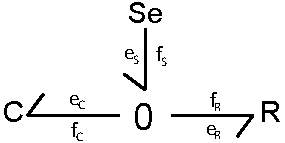
\includegraphics{RC_bondgraph.pdf}
\caption{A simple bond graph}
\end{figure}
We wish to use this bond graph of as a simple example of how to generate model equations.
\vspace{10pt}

\begin{center}
\emph{We need the constitutive relations for the components}.
\end{center}

\begin{figure}
\end{figure}
\end{frame}
\begin{frame}
\frametitle{0-Junction}
The 0-Junction, or common effort junction, conservatively balances power across many bonds, with equal effort.
\begin{figure}
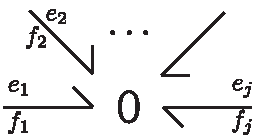
\includegraphics{nport-0.pdf}
\end{figure}
\only<1>{
Conservation of Energy implies $\sum_{i=1}^j e_i f_i = 0$.
\vspace{10pt}

Equal effort implies $e_1=e_2 = \ldots = e_j$, hence $\sum_{i=1}^j f_i = 0$.
\vspace{10pt}
\begin{center}
\emph{This is Kirchoff's Current Law!}
\end{center}}
\only<2>{
	\[
\Phi_\text{0}(e_1,f_1,e_2,f_2,\ldots, e_j,f_j) = \left(\begin{matrix}
	e_1 -e_2\\
	\ldots\\
	e_{j-1} - e_j\\
	f_1 + f_2 + \ldots + f_j 
\end{matrix}\right) = 0
\] 

}
\end{frame}
\begin{frame}
\frametitle{R component}
The R component dissipates power proportionally to $f^2$ (or $e^2$).
\begin{figure}
	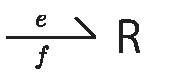
\includegraphics{oneport-R.pdf}
\end{figure}
The constitutive relation is given by
\[
\Phi_\text{R}(e,f) = e - Rf = 0.
\]
\vspace{10pt}

\begin{center}
\emph{This is both Ohms law and Newtonian friction.}
\end{center}
\end{frame}
\begin{frame}
\frametitle{C component}
The C component stores potential energy.
\begin{figure}
	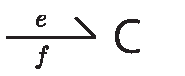
\includegraphics{oneport-C.pdf}
\end{figure}
The constitutive relation is given by
\[
\Phi_\text{C}(e,f) = Ce - \int f \df{t} = 0.
\]
\vspace{10pt}

\begin{center}
\emph{This is Hooke's law and the ideal capacitor relation.}
\end{center}
\end{frame}
\begin{frame}
\frametitle{Se component}
The ideal effort source provides power into the system.
\begin{figure}
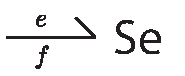
\includegraphics{oneport-Se.pdf}
\end{figure}
Here $f$ is allowed to vary freely and effort is specified by a control variable $u$
\[
\Phi_\text{Se}(e,f) = e - u.
\]

\end{frame}
\begin{frame}
\frametitle{Table of Constitutive Relations}
\begin{scriptsize}
	\begin{minipage}[c][\textheight][t]{0.4\textwidth}
		\vspace{0.75cm}
		\begin{tabular}{| l | c |}
			Node & Constitutive Relation\\
			\hline
			& \\
			R & $\Phi_\text{R} = e -Rf$\\
			L & $\Phi_\text{L} = \int e\df{t} - Lf$\\
			C & $\Phi_\text{C} = Ce - \int f \df{t}$\\&\\
			Se & $\Phi_\text{Se} = e - u$\\
			Sf & $\Phi_\text{Sf} = f - u$\\&\\
			TF & $\Phi_\text{TF} =\left(\begin{matrix}
			e_2 - \rho e_1 \\
			f_2 +\frac{1}{\rho}f_1
			\end{matrix} \right)$\\
			GY & $\Phi_\text{GY} =\left(\begin{matrix}
			e_2 - \rho f_1 \\
			f_2 +\frac{1}{\rho}e_1
			\end{matrix} \right)$\\&\\
			Ce & $\Phi_\text{Ce} = e -\alpha - \beta\ln \int f\df{t}$
		\end{tabular}
	\end{minipage}\hfill
	\begin{minipage}[c][\textheight][t]{0.45\textwidth}
		\vspace{0.75cm}
		\begin{tabular}{| l | c |}
			Node & Constitutive Relation\\
			\hline
			&\\
			0 &$	\Phi_\text{0} = \left(\begin{matrix}
			e_1 -e_2\\
			\ldots\\
			e_{j-1} - e_j\\
			f_1 + f_2 + \ldots + f_j 
			\end{matrix}\right)$\\
			&
			\\
			1&$	\Phi_\text{1} = \left(\begin{matrix}
			f_1 -f_2\\
			\ldots\\
			f_{j-1} - f_j\\
			e_1 + e_2 + \ldots + e_j 
			\end{matrix}\right)$\\ &\\
			Re & $\Phi_\text{Re}= \left( 
			\begin{matrix}
			\kappa \e^{\alpha e_1} - \kappa \e^{\alpha e_2} - f_1\\
			f_1 + f_2
			\end{matrix}
\right)$\\&
		\end{tabular}
	\end{minipage}

\end{scriptsize}
%Ce and Re are biochemical components~\cite{Gaw2014}
\end{frame}
\begin{frame}
\frametitle{Putting it Together}
\begin{small}
\begin{minipage}{0.4\textwidth}
\begin{figure}
	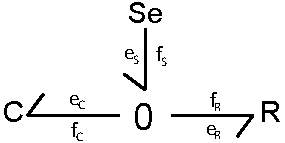
\includegraphics[width=\textwidth]{RC_bondgraph.pdf}
\end{figure}
\end{minipage}
\begin{minipage}{0.57\textwidth}
\begin{eqnarray}
\Phi_\text{C} &=& Ce_C - \int f_C \df{t}\\
\Phi_\text{R} &=& e_R - Rf_R\\
\Phi_\text{Se} & =& e_S - u\\
\Phi_\text{0} &=&
\left(\begin{matrix}
e_S  - e_C\\
e_S - e_R\\
f_S  + (- f_C) +  (-f_R)
\end{matrix}\right)
\end{eqnarray}
\end{minipage}
Goal: Find $f_S$.\\
Notice that (3) and (4) give $u = e_S =e_R = e_C$ which when combined with (1) and (2) gives $f_C = C^{-1}\dot{u}$ and $f_R = R^{-1}u$ respectively.\\
\vspace{5pt}

The last equation of (4) then gives our result:
\[
f_S = \left(\frac{1}{R} + \frac{1}{C}\D{}{t}\right)u.
\]
\end{small}
\end{frame}

\begin{frame}
\frametitle{In Review}
Hopefully I've convinced you that bond graphs :
\begin{itemize}
	\item `naturally' model energy distribution across networks
	\item are very useful for modelling multi-domain systems.
	\item conserve energy when connecting network subsystems.
\end{itemize}
\vspace{22pt}

Network subsystems can be:
\begin{itemize}
	\item derived from first principles,
	\item defined phenomenologically, 
	\item constructed hierarchically.
\end{itemize}
\emph{This makes for a powerful, multi-domain and multi-scale modelling tool.}
\end{frame}
\section{Bond Graphs @ SBL}
\begin{frame}
\frametitle{Bond Graphs @ SBL}
Bond Graph researchers at the SBL:
\begin{itemize}
	\item Prof. Edmund Crampin (Director)
	\item Prof. Peter Gawthrop
	\item Michael Pan
	\item PC
\end{itemize}
\begin{small}

Website: \url{https://systemsbiologylaboratory.org/}\\
	\vspace{10pt}
	
At the Systems Biology Lab we aim to build `comprehensive' models of cells, with heart cells as our working model.\\
\vspace{10pt}

Bond Graphs play a central role in ensuring our models remain physical.
\end{small}
\end{frame}


\begin{frame}
\frametitle{Cellular Biochemistry and Metabolism}

Prof. Peter Gawthrop is working on bond graph models of cellular biochemistry and metabolism.\\
\vspace{10pt}

Website: \url{www.gawthrop.net}
\vspace{10pt}

Recent Publications:
\begin{itemize}
	\itemsep1em
	\item  P.J. Gawthrop, E.J. Crampin. 2017. \emph{Energy-based Analysis of Biomolecular Pathways}
	Proceedings of the Royal Society A, 473:20160825.
	\item P. Gawthrop. 2017. \emph{Computing Biomolecular System Steady-states.}
	 IEEE Transactions on NanoBioscience, vol. PP, no. 99, pp. 1-1. 
\end{itemize}


\end{frame}
\begin{frame}
\frametitle{Electrophysiology}
Michael Pan is working on bond graph approaches in electrophysiology and ionic homeostasis. \\
\vspace{10pt}

You'll hear more from Michael later in this session.\\
\vspace{10pt}

Forthcoming publications:
\begin{itemize}
	\itemsep1em
	\item M. Pan, P.J. Gawthrop, J. Cursons, K. Tran, E.J. Crampin. \emph{Bond graph modelling of the cardiac action potential: Implications for drift and non-unique steady states}.
	\item M. Pan, P.J. Gawthrop, J. Cursons, K. Tran, E.J. Crampin.
	\emph{The cardiac Na+/K+ ATPase: An updated, thermodynamically consistent model}.
\end{itemize}
\end{frame}
\begin{frame}
\frametitle{Synthetic Biology}
I joined the System Biology Lab in November, 2017 and am working on
\begin{itemize}
	\itemsep1em
	\item Bond graph techniques for rational design in synthetic biology and bioengineering.
	\item Improving the bond graph modelling tool-chain. 
	\item Investigating the connection between bond graphs, Hamiltonian mechanics, network dynamics, and operator theory applications to stochastic mechanics.
\end{itemize}
\vspace{10pt}


Website: \url{https://github.com/peter-cudmore/}

\end{frame}



\begin{frame}
\frametitle{Thanks}
{\small
Thanks to
\begin{itemize}
		\itemsep1em
	\item Prof. Edmund Crampin and Prof. Peter Gawthrop
	\item Andre, the CellML workshop organisers and the Auckland Bioengineering Institute
\item Systems Biology Laboratory, School of Mathematics and Statistics and Department of Biomedical Engineering, University of Melbourne, Parkville, Victoria 3010
\item ARC Centre of Excellence in Convergent Bio-Nano Science and Technology,
Melbourne school of Engineering, 
University of Melbourne, Parkville, Victoria 3010
\end{itemize}
}
\end{frame}
\begin{frame}
\frametitle{References}
{\tiny
	\begin{thebibliography}{6}
		\bibitem{Feynman1961} Feynman, Richard. \emph{The Feynman Lectures on Physics; Volume 1.} U.S.A: Addison Wesley, 1964. ISBN 0-201-02115-3.
		\bibitem{Karnopp} Karnopp, Dean C. and Margolis Donald L. and Rosenberg, Ronald C. \emph{System Dynamics: a Unified Approach}, Wiley, New York, 1990.
		\bibitem{baez} Baez, John. 2010. \emph{This Weeks Finds in Mathematical Physics (Week 289).} \url{http://math.ucr.edu/home/baez/week289.html}
		\bibitem{Gaw2017a}  P.J. Gawthrop, E.J. Crampin. 2017. \emph{Energy-based Analysis of Biomolecular Pathways}\\
		Proceedings of the Royal Society A, 473:20160825.
		\bibitem{Gaw2017b} P. Gawthrop. 2017. \emph{Computing Biomolecular System Steady-states.}\\
		IEEE Transactions on NanoBioscience, vol. PP, no. 99, pp. 1-1. 
		\bibitem{Gaw2014} P.J. Gawthrop, E.J. Crampin. 2014. \emph{Energy-based analysis of biochemical cycles using bond graphs}\\
		Proceedings of the Royal Society A, 470:20140459.
		\bibitem{payter2000} Payner, H.M. 2000. \emph{The Gestation and Birth of Bond Graphs} \url{http://www.me.utexas.edu/\~longoria/paynter/hmp/Bondgraphs.html}
\end{thebibliography}}
\end{frame}
\end{document}